\documentclass[11pt,a4paper]{book}

% bibliography on the same page
% https://tex.stackexchange.com/questions/74296/to-have-no-pagebreak-before-bibliography
\usepackage{etoolbox}
\patchcmd{\thebibliography}{\chapter*}{\section*}{}{}

\usepackage{ceteiep_dsa_notes_whitebg}

\addto\captionsgreek{\renewcommand{\chaptername}{Εργαστήριο}}

\title{Δομές Δεδομένων και Αλγόριθμοι \\ ΜΕΡΟΣ B' \\ Εργαστήριο (C++)\\ Τ.Ε.Ι. Ηπείρου - Τμήμα Μηχανικών Πληροφορικής Τ.Ε.}
\author{Χρήστος Γκόγκος }
\date{Άρτα - 2017}

\begin{document}
% \frontmatter
\maketitle
% \tableofcontents
\mainmatter

\setcounter{chapter}{3} 
% Εργαστήριο 4
\chapter{Γραμμικές λίστες, λίστες της STL}
\section{Εισαγωγή}
Οι γραμμικές λίστες είναι δομές δεδομένων που επιτρέπουν την αποθήκευση και την προσπέλαση στοιχείων έτσι ώστε τα στοιχεία να βρίσκονται σε μια σειρά με σαφώς ορισμένη την έννοια της θέσης καθώς και το ποιο στοιχείο προηγείται και ποιο έπεται καθενός. Σε χαμηλού επιπέδου γλώσσες προγραμματισμού όπως η C η υλοποίηση γραμμικών λιστών είναι ευθύνη του προγραμματιστή. Από την άλλη μεριά, γλώσσες υψηλού επιπέδου όπως η C++, η Java, η Python κ.α. προσφέρουν έτοιμες υλοποιήσεις γραμμικών λιστών. Ωστόσο, η γνώση υλοποίησης των συγκεκριμένων δομών (όπως και άλλων) αποτελεί βασική ικανότητα η οποία αποκτά ιδιαίτερη χρησιμότητα όταν ζητούνται εξειδικευμένες υλοποιήσεις. Για το λόγο αυτό στο συγκεκριμένο εργαστήριο θα παρουσιαστούν οι υλοποιήσεις γραμμικών λιστών αλλά και οι ενσωματωμένες δυνατότητες της C++ μέσω της STL.

\section{Γραμμικές λίστες}
Υπάρχουν δύο βασικοί τρόποι αναπαράστασης γραμμικών λιστών, η στατική αναπαράσταση η οποία γίνεται με τη χρήση πινάκων και η αναπαράσταση με συνδεδεμένη λίστα η οποία γίνεται με τη χρήση δεικτών. 

\subsection{Στατικές γραμμικές λίστες}
Στη στατική γραμμική λίστα τα δεδομένα αποθηκεύονται σε ένα πίνακα. Κάθε στοιχείο της στατικής λίστας μπορεί να προσπελαστεί με βάση τη θέση του στον ίδιο σταθερό χρόνο με όλα τα άλλα στοιχεία άσχετα με τη θέση στην οποία βρίσκεται (τυχαία προσπέλαση). Ο κώδικας υλοποίησης μιας στατικής λίστας με μέγιστη χωρητικότητα 50.000 στοιχείων παρουσιάζεται στη συνέχεια.

\lstinputlisting[caption = Υλοποίηση στατικής γραμμικής λίστας (static\_list.cpp)]{lab04/static_list.cpp}

\lstinputlisting[caption = Παράδειγμα με στατική γραμμική λίστα (list1.cpp)]{lab04/list1.cpp}

\lstinputlisting[style=DOS]{lab04/list1.out}


\subsection{Συνδεδεμένες γραμμικές λίστες}
\lstinputlisting[caption = Υλοποίηση συνδεδεμένης γραμμικής λίστας (linked\_list.cpp)]{lab04/linked_list.cpp}

\lstinputlisting[caption = Παράδειγμα με συνδεδεμένη γραμμική λίστα (list2.cpp)]{lab04/list2.cpp}

\lstinputlisting[style=DOS]{lab04/list2.out}

\subsection{Γραμμικές λίστες της STL}
\subsubsection{list}
\subsubsection{forwardlist}
\subsubsection{vector}


\section{Παραδείγματα}
\subsection{Παράδειγμα 1}
Γράψτε ένα πρόγραμμα που να ελέγχεται από το ακόλουθο μενού και να πραγματοποιεί τις λειτουργίες που περιγράφονται σε μια απλά συνδεδεμένη λίστα με ακεραίους
\begin{enumerate}
\item 1. Show items
\item 2. Insert item at given position 
\item 3. Delete item at given position
\item 4. Delete item
\item 5. Exit
\end{enumerate}

\subsection{Παράδειγμα 2}
Έστω μια υποθετική τράπεζα. Για κάθε πελάτη έστω ότι η τράπεζα διατηρεί σε ένα αρχείο το ονοματεπώνυμο του και το υπόλοιπο του λογαριασμού του. Για τις ανάγκες της άσκησης θα πρέπει να δημιουργηθούν τυχαίοι πελάτες ως εξής: το όνομα κάθε πελάτη να αποτελείται από 10 γράμματα που θα επιλέγονται με τυχαίο τρόπο από τα γράμματα της αγγλικής αλφαβήτου και το δε υπόλοιπο κάθε πελάτη να είναι ένας τυχαίος αριθμός από το 0 μέχρι το 5.000. 
Θα παρουσιαστούν τέσσερις εκδόσεις του ίδιου προγράμματος. Η μεν πρώτη θα υλοποιείται με στατική λίστα,  η δεύτερη με συνδεδεμένη λίστα η τρίτη με τη στατική γραμμική λίστα της C++, std::vector και η τέταρτη με τη συνδεδεμένη λίστα της C++, std::list. Και στις τέσσερις περιπτώσεις το πρόγραμμα θα πραγματοποιεί τις ακόλουθες λειτουργίες:

\begin{itemize}[noitemsep]
\item Θα δημιουργεί μια λίστα με 40.000 τυχαίους πελάτες.
\item Θα υπολογίζει το άθροισμα των υπολοίπων από όλους τους πελάτες που το όνομά τους ξεκινά με το χαρακτήρα Α.
\item Θα προσθέτει για κάθε πελάτη που το όνομά του ξεκινά με το χαρακτήρα Α στην αμέσως επόμενη θέση έναν πελάτη με όνομα το αντίστροφο όνομα του πελάτη και το ίδιο υπόλοιπο λογαριασμού.
\item Θα διαγράφει όλους τους πελάτες που το όνομά τους ξεκινά με το χαρακτήρα Β.
\end{itemize}

\lstinputlisting[caption = Παράδειγμα με συνδεδεμένη γραμμική λίστα (lab04\_ex1.cpp)]{lab04/lab04_ex1.cpp}

\lstinputlisting[style=DOS]{lab04/lab04_ex1.out}

\section{Ασκήσεις}
\begin{enumerate}
\item Έστω η συνδεδεμένη λίστα που παρουσιάστηκε στον κώδικα ΧΧ. Προσθέστε μια συνάρτηση που μια λίστα ακεραίων στην οποία τα στοιχεία της είναι ταξινομημένα από το μικρότερο στο μεγαλύτερο να προσθέτει ένα ακόμα στοιχείο στην κατάλληλη θέση έτσι ώστε η λίστα να παραμένει ταξινομημένη.
\item Έστω η συνδεδεμένη λίστα που παρουσιάστηκε στον κώδικα ΧΧ. Προσθέστε μια συνάρτηση που να αντιστρέφει τη λίστα.
\item Υλοποιήστε τους κώδικες της στατικής ΧΧ και της συνδεδεμένης λίστας ΧΧ με κλάσεις. Τροποποιήστε το παράδειγμα 1 έτσι ώστε να δίνεται επιλογή στο χρήστη να χρησιμοποιήσει είτε τη στατική είτε τη συνδεδεμένη λίστα προκειμένου να εκτελέσει τις ίδιες λειτουργίες πάνω σε μια λίστα. 
\item Υλοποιήστε μια κυκλικά συνδεδεμένη λίστα. Η κυκλική λίστα είναι μια απλά συνδεδεμένη λίστα στην οποία το τελευταίο στοιχείο της λίστας δείχνει στο πρώτο στοιχείο της λίστας. Η υλοποίηση θα πρέπει να συμπεριλαμβάνει και δύο δείκτες, έναν που να δείχνει στο πρώτο στοιχείο της λίστας και έναν που να δείχνει στο τελευταίο στοιχείο της λίστας. Προσθέστε τις απαιτούμενες λειτουργίες έτσι ώστε η λίστα να παρέχονται οι ακόλουθες λειτουργίες: εμφάνιση λίστας, εισαγωγή στοιχείου, διαγραφή στοιχείου, εμφάνιση πλήθους στοιχείων, εύρεση στοιχείου. Γράψτε πρόγραμμα που να δοκιμάζει τις λειτουργίες της λίστας.
\end{enumerate}


\begin{thebibliography}{9}

\bibitem{hackernoon}
Stable Sorting, \href{https://hackernoon.com/stable-sorting-677453884792}{https://hackernoon.com/stable-sorting-677453884792}

\end{thebibliography}



% Εργαστήριο 5
\chapter{Στοίβες και ουρές, οι δομές στοίβα και ουρά στην STL}
\section{Εισαγωγή}
Οι στοίβες και οι ουρές αποτελούν απλές δομές δεδομένων που είναι ιδιαίτερα χρήσιμες στην επίλυση αλγοριθμικών προβλημάτων. Η στοίβα είναι μια λίστα στοιχείων στην οποία τα νέα στοιχεία τοποθετούνται στην κορυφή και όταν πρόκειται να αφαιρεθεί ένα στοιχείο αυτό πάλι συμβαίνει από την κορυφή των στοιχείων της στοίβας. Από την άλλη μεριά η ουρά είναι επίσης μια λίστα στοιχείων στην οποία όμως οι εισαγωγές γίνονται στο πίσω άκρο της ουράς ενώ οι εξαγωγές πραγματοποιούνται από το εμπρός άκρο της ουράς. Στο εργαστήριο αυτό θα παρουσιαστούν υλοποιήσεις της στοίβας και της ουράς. Επιπλέον, θα παρουσιαστούν οι δομές της STL std::stack και std::queue.
Ο κώδικας όλων των παραδειγμάτων βρίσκεται στο \href{https://github.com/chgogos/ceteiep_dsa}{https://github.com/chgogos/ceteiep\_dsa}.

\section{Στοίβα}
Η στοίβα (stack) είναι μια ειδική περίπτωση γραμμικής λίστας στην οποία οι εισαγωγές και οι διαγραφές επιτρέπονται μόνο από το ένα άκρο. Συνήθως αυτό το άκρο λέγεται κορυφή (top). Πρόκειται για μια δομή στην οποία οι εισαγωγές και οι εξαγωγές γίνονται σύμφωνα με το μοντέλο τελευταίο μέσα πρώτο έξω (LIFO=Last In First Out).

Στη συνέχεια παρουσιάζεται μια υλοποίηση στοίβας που χρησιμοποιεί για την αποθήκευση των στοιχείων της έναν πίνακα. Εναλλακτικά, στη θέση του πίνακα μπορεί να χρησιμοποιηθεί συνδεδεμένη λίστα. Μια υλοποίηση στη γλώσσα C μπορεί να βρεθεί στην αναφορά \cite{tcc_stack_linked_list}. 
\lstinputlisting[caption = Υλοποίηση στοίβας (stack\_oo.cpp),label=lst:stack_oo.cpp]{lab05/stack_oo.cpp}

\lstinputlisting[style=DOS]{lab05/stack_oo.out}

\section{Ουρά}
Η ουρά (queue) είναι μια ειδική περίπτωση γραμμικής λίστας στην οποία επιτρέπονται εισαγωγές στο πίσω άκρο της και εξαγωγές από το εμπρός άκρο της μόνο. Τα δύο αυτά άκρα συνήθως αναφέρονται ως πίσω (rear) και εμπρός (front) αντίστοιχα. Η ουρά είναι μια δομή στην οποία οι εισαγωγές και οι εξαγωγές γίνονται σύμφωνα με το μοντέλο πρώτο μέσα πρώτο έξω (FIFO=First In First Out).

Στη συνέχεια παρουσιάζεται μια υλοποίηση ουράς στην οποία τα δεδομένα της τοποθετούνται σε έναν πίνακα (εναλλακτικά θα μπορούσε να είχε χρησιμοποιηθεί μια άλλη δομή όπως για παράδειγμα η συνδεδεμένη λίστα). Ο πίνακας λειτουργεί κυκλικά, δηλαδή όταν συμπληρωθεί και εφόσον υπάρχουν διαθέσιμες κενές θέσεις στην αρχή του πίνακα, τα νέα στοιχεία που πρόκειται να εισαχθούν στην ουρά τοποθετούνται εκεί.

\lstinputlisting[caption = Υλοποίηση ουράς (queue\_oo.cpp),label=lst:queue_oo.cpp]{lab05/queue_oo.cpp}

\lstinputlisting[style=DOS]{lab05/queue_oo.out}

\section{Οι δομές στοίβα και ουρά στην STL}
Οι δομές std::stack και std::queue έχουν υλοποιηθεί στην STL ως container adaptors δηλαδή κλάσεις που χρησιμοποιούν εσωτερικά ένα άλλο container και παρέχουν ένα συγκεκριμένο σύνολο από λειτουργίες που επιτρέπουν την προσπέλαση και την τροποποίηση των στοιχείων τους. Το εσωτερικό container μπορεί να είναι κάποιο από τα containers της STL: vector, list, dequeue ή οποιοδήποτε container που υποστηρίζει τις λειτουργίες: empty, size, back, push\_back και pop\_back.
\subsection{std::stack}
Τυπικές λειτουργίες που παρέχει η std::stack είναι οι ακόλουθες:
\begin{itemize}[noitemsep]
\item empty, ελέγχει αν η στοίβα είναι άδεια.
\item size, επιστρέφει το μέγεθος της στοίβας.
\item top, προσπελαύνει το στοιχείο που βρίσκεται στη κορυφή της στοίβας (χωρίς να το αφαιρεί).
\item push, ωθεί ένα στοιχείο στη κορυφή της στοίβας
% \item emplace, δημιουργεί και εισάγει ένα στοιχείο στη κορυφή της στοίβας.
\item pop, αφαιρεί το στοιχείο που βρίσκεται στη κορυφή της στοίβας.
% \item swap, αντιμεταθέτει τα περιεχόμενα από δύο στοίβες.
\end{itemize}

Ένα παράδειγμα χρήσης της std::stack παρουσιάζεται στη συνέχεια.

\lstinputlisting[caption = Παράδειγμα χρήσης της std::stack (stl\_stack\_example.cpp)]{lab05/stl_stack_example.cpp}

\lstinputlisting[style=DOS]{lab05/stl_stack_example.out}


\subsection{std::queue}
Τυπικές λειτουργίες που παρέχει η std::queue είναι οι ακόλουθες:
\begin{itemize}[noitemsep]
\item empty, ελέγχει αν η ουρά είναι άδεια.
\item size, επιστρέφει το μέγεθος της ουράς.
\item front, προσπελαύνει το στοιχείο που βρίσκεται στο εμπρός άκρο της ουράς (χωρίς να το αφαιρεί).
\item back, προσπελαύνει το στοιχείο που βρίσκεται στο πίσω άκρο της ουράς (χωρίς να το αφαιρεί).
\item push, ωθεί ένα στοιχείο στο πίσω άκρο της ουράς
\item pop, αφαιρεί το στοιχείο που βρίσκεται στο εμπρός άκρο της ουράς.
\end{itemize}

Ένα παράδειγμα χρήσης της std::queue παρουσιάζεται στη συνέχεια.
\lstinputlisting[caption = Παράδειγμα χρήσης της std::queue (stl\_queue\_example.cpp)]{lab05/stl_queue_example.cpp}

\lstinputlisting[style=DOS]{lab05/stl_queue_example.out}

\section{Παραδείγματα}
\subsection{Παράδειγμα 1}
Να γραφεί πρόγραμμα που να δέχεται μια φράση ως παράμετρο γραμμής εντολών και να εμφανίζει το εάν είναι παλινδρομική ή όχι. Μια φράση είναι παλινδρομική όταν διαβάζεται η ίδια από αριστερά προς τα δεξιά και από δεξιά προς τα αριστερά.
\lstinputlisting[caption = Έλεγχος παλινδρομικής φράσης (lab05\_ex1.cpp)]{lab05/lab05_ex1.cpp}

\lstinputlisting[style=DOS]{lab05/lab05_ex1.out}

\subsection{Παράδειγμα 2}
Να γραφεί πρόγραμμα που να δέχεται ένα δυαδικό αριθμό ως λεκτικό και να εμφανίζει την ισοδύναμη δεκαδική του μορφή.
\lstinputlisting[caption = Μετατροπή δυαδικού σε δεκαδικό (lab05\_ex2.cpp)]{lab05/lab05_ex2.cpp}

\lstinputlisting[style=DOS]{lab05/lab05_ex2.out}

% \subsection{Παράδειγμα 3}

\section{Ασκήσεις}
\begin{enumerate}
\item Να υλοποιηθεί η δομή της ουράς χρησιμοποιώντας αντικείμενα στοίβας (std::stack) και τις λειτουργίες που επιτρέπονται σε αυτά. Υλοποιήστε τις λειτουργίες της ουράς empty, size, enqueue, dequeue και front.
\item Να υλοποιηθεί η δομή της στοίβας χρησιμοποιώντας αντικείμενα ουράς (std::queue) και τις λειτουργίες που επιτρέπονται σε αυτά. Υλοποιήστε τις λειτουργίες της στοίβας empty, size, push, pop και top.
\end{enumerate}

\begin{thebibliography}{9}
\bibitem{tcc_stack_linked_list}
Tech Crash Course,  C Program to Implement a Stack using Singly Linked List, \href{http://www.techcrashcourse.com/2016/06/c-program-implement-stack-using-linked-list.html}{http://www.techcrashcourse.com/2016/06/c-program-implement-stack-using-linked-list.html}

\end{thebibliography}



% Εργαστήριο 6
\chapter{Σωροί μεγίστων και σωροί ελαχίστων, η ταξινόμηση heapsort, ουρές προτεραιότητας στην STL}
\chaptermark{Σωροί μεγίστων, ελαχίστων, heapsort, std::priority\_queue}
\section{Εισαγωγή}
Οι σωροί επιτρέπουν την οργάνωση των δεδομένων με τέτοιο τρόπο έτσι ώστε το μεγαλύτερο στοιχείο να είναι συνεχώς προσπελάσιμο σε σταθερό χρόνο. Η δε λειτουργίες της εισαγωγής νέων τιμών στη δομή και της διαγραφή της μεγαλύτερης τιμής πραγματοποιούνται ταχύτατα. Σε αυτό το εργαστήριο θα παρουσιαστεί η υλοποίηση ενός σωρού μεγίστων και ο σχετικός με τη δομή αυτή αλγόριθμος ταξινόμησης, heapsort. Επιπλέον, θα παρουσιαστεί η δομή std::priority\_queue που υλοποιεί στην STL της C++ τους σωρούς μεγίστων και ελαχίστων. Ο κώδικας όλων των παραδειγμάτων βρίσκεται στο \href{https://github.com/chgogos/ceteiep_dsa}{https://github.com/chgogos/ceteiep\_dsa}.

\section{Σωροί}
Ο σωρός είναι μια μερικά ταξινομημένη δομή δεδομένων. Υπάρχουν δύο βασικά είδη σωρών: ο σωρός μεγίστων (MAXHEAP) και ο σωρός ελαχίστων (MINHEAP). Οι ιδιότητες των σωρών που θα περιγραφούν στη συνέχεια αφορούν τους σωρούς μεγίστων αλλά αντίστοιχες ιδιότητες ισχύουν και για τους σωρούς ελαχίστων. Ειδικότερα, ένας σωρός μεγίστων υποστηρίζει ταχύτατα τις ακόλουθες λειτουργίες:
\begin{itemize}[noitemsep]
\item Εύρεση του στοιχείου με τη μεγαλύτερη τιμή κλειδιού.
\item Διαγραφή του στοιχείου με τη μεγαλύτερη τιμή κλειδιού.
\item Εισαγωγή νέου κλειδιού στη δομή.
\end{itemize}

Ένας σωρός μπορεί να θεωρηθεί ως ένα δυαδικό δένδρο για το οποίο ισχύουν οι ακόλουθοι δύο περιορισμοί:
\begin{itemize}[noitemsep]
\item	{\em Πληρότητα}: το δυαδικό δένδρο είναι συμπληρωμένο, δηλαδή όλα τα επίπεδά του είναι πλήρως συμπληρωμένα εκτός πιθανά από το τελευταίο (χαμηλότερο) επίπεδο στο οποίο μπορούν να λείπουν μόνο κάποια από τα δεξιότερα φύλλα.
\item	{\em Κυριαρχία γονέα}: το κλειδί σε κάθε κορυφή είναι μεγαλύτερο ή ίσο από τα κλειδιά των παιδιών (σε MAXHEAP).
\end{itemize}

Ένας σωρός μπορεί να υλοποιηθεί με ένα πίνακα καταγράφοντας στον πίνακα στη σειρά τα στοιχεία του δυαδικού δένδρου από αριστερά προς τα δεξιά και από πάνω προς τα κάτω (σχήμα \ref{fig:heap2}). Μερικές σημαντικές ιδιότητες οι οποίες προκύπτουν εφόσον τηρηθεί ο παραπάνω τρόπος αντιστοίχισης των στοιχείων του δένδρου στα στοιχεία του  πίνακα είναι οι ακόλουθες:
\begin{itemize}[noitemsep]
\item	Στον πίνακα, τα κελιά γονείς βρίσκονται στις πρώτες $\lfloor{\frac{n}{2}}\rfloor$ θέσεις ενώ τα φύλλα καταλαμβάνουν τις υπόλοιπες θέσεις. 
\item	Στον πίνακα, τα παιδιά για κάθε κλειδί στις θέσεις $i$ από 1 μέχρι και $\lfloor{\frac{n}{2}}\rfloor$ βρίσκονται στις θέσεις $2*i$ και $2*i + 1$.
\item	Στον πίνακα, ο γονέας για κάθε κλειδί στις θέσεις $i$ από 2 μέχρι και $n$ βρίσκεται στη θέση $\lfloor{\frac{i}{2}}\rfloor$.
\end{itemize}


\begin{figure}[ht]
\centering
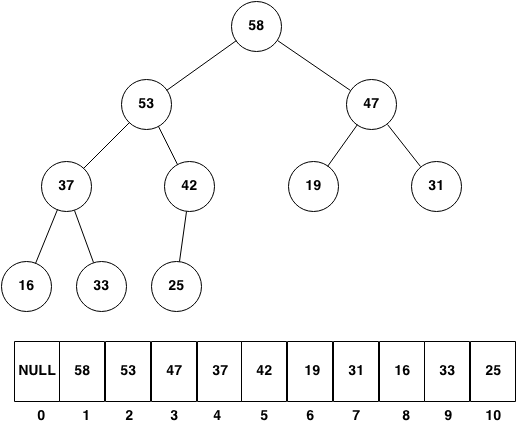
\includegraphics[width=100mm]{heap2.png}
\caption{Αναπαράσταση ενός σωρού μεγίστων ως πίνακα}
\label{fig:heap2}
\end{figure}

Για το παράδειγμα του σχήματος ισχύουν τα ακόλουθα:
\begin{itemize}
\item Οι κόμβοι που είναι γονείς (έχουν τουλάχιστον ένα παιδί) βρίσκονται στις θέσεις από 1 μέχρι και 5.
\item Οι κόμβοι που είναι φύλλα βρίσκονται στις θέσεις από 6 μέχρι και 10.
\item Ο γονέας στη θέση 1 (η τιμή 58) έχει παιδιά στις θέσεις $2*1=2$ (τιμή 53) και $2*1+1=3$ (τιμή 47).
\item Ο γονέας στη θέση 2 (η τιμή 53) έχει παιδιά στις θέσεις $2*2=4$ (τιμή 37) και $2*2+1=5$ (τιμή 42).
\item Ο γονέας στη θέση 3 (η τιμή 47) έχει παιδιά στις θέσεις $2*3=6$ (τιμή 19) και $2*3+1=7$ (τιμή 31).
\item Ο γονέας στη θέση 4 (η τιμή 37) έχει παιδιά στις θέσεις $2*4=8$ (τιμή 16) και $2*4+1=9$ (τιμή 33).
\item Ο γονέας στη θέση 5 (η τιμή 42) έχει παιδιά στις θέσεις $2*5=10$ (τιμή 25).
\item Ο κόμβος παιδί στη θέση 2 (η τιμή 53) έχει γονέα στη θέση $\lfloor{\frac{2}{2}}\rfloor=1$ (τιμή 58).
\item Ο κόμβος παιδί στη θέση 3 (η τιμή 47) έχει γονέα στη θέση $\lfloor{\frac{3}{2}}\rfloor=1$ (τιμή 58).
\item Ο κόμβος παιδί στη θέση 4 (η τιμή 37) έχει γονέα στη θέση $\lfloor{\frac{4}{2}}\rfloor=2$ (τιμή 53).
\item Ο κόμβος παιδί στη θέση 5 (η τιμή 42) έχει γονέα στη θέση $\lfloor{\frac{5}{2}}\rfloor=2$ (τιμή 53).
\item Ο κόμβος παιδί στη θέση 6 (η τιμή 19) έχει γονέα στη θέση $\lfloor{\frac{6}{2}}\rfloor=3$ (τιμή 47).
\item Ο κόμβος παιδί στη θέση 7 (η τιμή 31) έχει γονέα στη θέση $\lfloor{\frac{7}{2}}\rfloor=3$ (τιμή 47).
\item Ο κόμβος παιδί στη θέση 8 (η τιμή 16) έχει γονέα στη θέση $\lfloor{\frac{8}{2}}\rfloor=4$ (τιμή 37).
\item Ο κόμβος παιδί στη θέση 9 (η τιμή 33) έχει γονέα στη θέση $\lfloor{\frac{9}{2}}\rfloor=4$ (τιμή 37).
\item Ο κόμβος παιδί στη θέση 10 (η τιμή 25) έχει γονέα στη θέση $\lfloor{\frac{10}{2}}\rfloor=5$ (τιμή 42).
\end{itemize}

\section{Υλοποίηση ενός σωρού}
Στη συνέχεια παρουσιάζεται η υλοποίηση ενός σωρού μεγίστων που περιέχει ακέραιες τιμές-κλειδιά.

\lstinputlisting[caption = Σωρός μεγίστων με κλειδιά ακέραιες τιμές (max\_heap.cpp)]{lab06/max_heap.cpp}

\subsubsection*{Οι συναρτήσεις δημιουργίας σωρού από πίνακα (heap\_bottom\_up και heapify)}
Ένας πίνακας μπορεί να μετασχηματιστεί ταχύτατα σε σωρό. Η διαδικασία ξεκινά από τον τελευταίο κόμβο γονέα του δένδρου (που βρίσκεται στη θέση $\lfloor{\frac{n}{2}}\rfloor$) και σταδιακά εφαρμόζεται μέχρι να φτάσει στον κόμβο στη θέση 1. Για καθένα από αυτούς τους κόμβους εξετάζεται από πάνω προς τα κάτω αν ισχύει η κυριαρχία γονέα και αν δεν ισχύει τότε γίνεται αντιμετάθεση με το μεγαλύτερο από τα παιδιά του επαναληπτικά. 

Ο ακόλουθος κώδικας χρησιμοποιεί τη συνάρτηση heap\_bottom\_up και μέσω αυτής τη συνάρτηση heapify προκειμένου να μετασχηματίσει έναν πίνακα ακεραίων σε σωρό μεγίστων. 
\lstinputlisting[caption = Δημιουργία σωρού από πίνακα με heapify (heap1.cpp)]{lab06/heap1.cpp}

\lstinputlisting[style=DOS]{lab06/heap1.out}

Στο σχήμα \ref{fig:heapify} παρουσιάζονται οι τιμές που έλαβε κάθε κόμβος του δένδρου προκειμένου να μετασχηματιστεί τελικά σε σωρό μεγίστων.

\begin{figure}[ht]
\centering
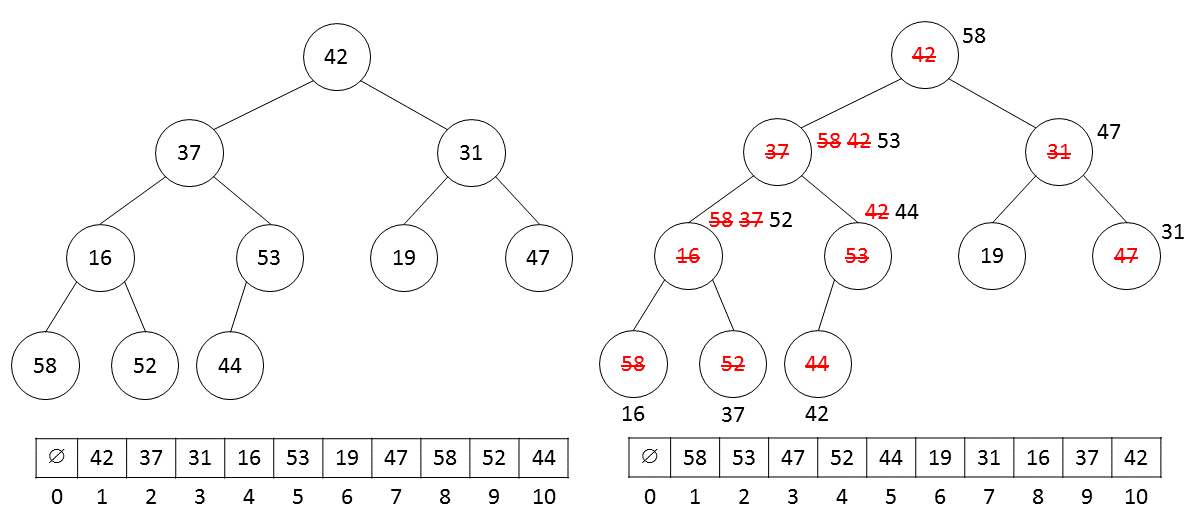
\includegraphics[width=150mm]{heapify.png}
\caption{Δημιουργία σωρού από πίνακα (heapify)}
\label{fig:heapify}
\end{figure}

\subsubsection*{Η συνάρτηση ελέγχου του εάν ο σωρός είναι άδειος (empty)}
Η συνάρτηση empty εξετάζει το μέγεθος του σωρού μέσω της μεταβλητής heap\_size. Αν η μεταβλητή heap\_size είναι μηδέν τότε επιστρέφει true, αλλιώς επιστρέφει false.

\subsubsection*{Η συνάρτηση λήψης της μεγαλύτερης τιμής από το σωρό (top)}
Καθώς η μεγαλύτερη τιμή βρίσκεται πάντα στη θέση 1 του πίνακα που διατηρεί τα δεδομένα του σωρού η συνάρτηση top απλά επιστρέφει την τιμή αυτή.

\subsubsection*{Η συνάρτηση εξαγωγής της μεγαλύτερης τιμής από το σωρό (pop)}
Η εξαγωγή της μεγαλύτερης τιμής γίνεται ως εξής. Το στοιχείο που βρίσκεται στην κορυφή του σωρού αντιμετατίθεται με το τελευταίο στοιχείο του σωρού. Στη συνέχεια το στοιχείο που έχει βρεθεί στην κορυφή του σωρού κατεβαίνει προς τα κάτω αν έχει παιδί που είναι μεγαλύτερό του πραγματοποιώντας αντιμετάθεση με το μεγαλύτερο στοιχείο από τα παιδιά του. Η διαδικασία επαναλαμβάνεται για τη νέα θέση του στοιχείου που αρχικά είχε μεταφερθεί στη κορυφή και μέχρι να ισχύσει ότι είναι μεγαλύτερο και από τα δύο παιδιά του. Στο σχήμα \ref{fig:heap_pop} παρουσιάζεται η εξαγωγή της κορυφαίας τιμής του σωρού.

\begin{figure}[ht!]
\centering
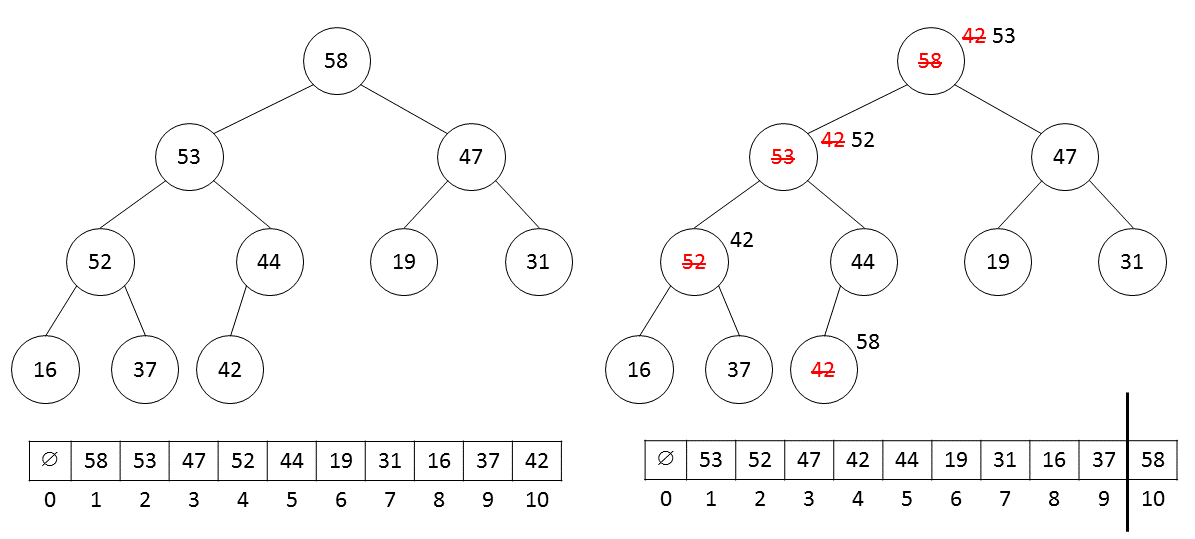
\includegraphics[width=150mm]{heap_pop.png}
\caption{Εξαγωγή της μεγαλύτερης τιμής του σωρού (pop)}
\label{fig:heap_pop}
\end{figure}

\subsubsection*{Η συνάρτηση εισαγωγής νέας τιμής στο σωρό (push)}
Η εισαγωγή ενός στοιχείου γίνεται ως φύλλο στη πρώτη διαθέσιμη θέση από πάνω προς τα κάτω και από δεξιά προς τα αριστερά. Το στοιχείο αυτό συγκρίνεται με το γονέα του και αν είναι μεγαλύτερο αντιμετατίθεται με αυτόν. Η διαδικασία συνεχίζεται μέχρι είτε να βρεθεί το νέο στοιχείο στην κορυφή είτε να ισχύει η κυριαρχία γονέα. Στο σχήμα \ref{fig:heap_push} παρουσιάζεται η εισαγωγή της τιμής 60 σε έναν σωρό μεγίστων.

\begin{figure}[H]
\centering
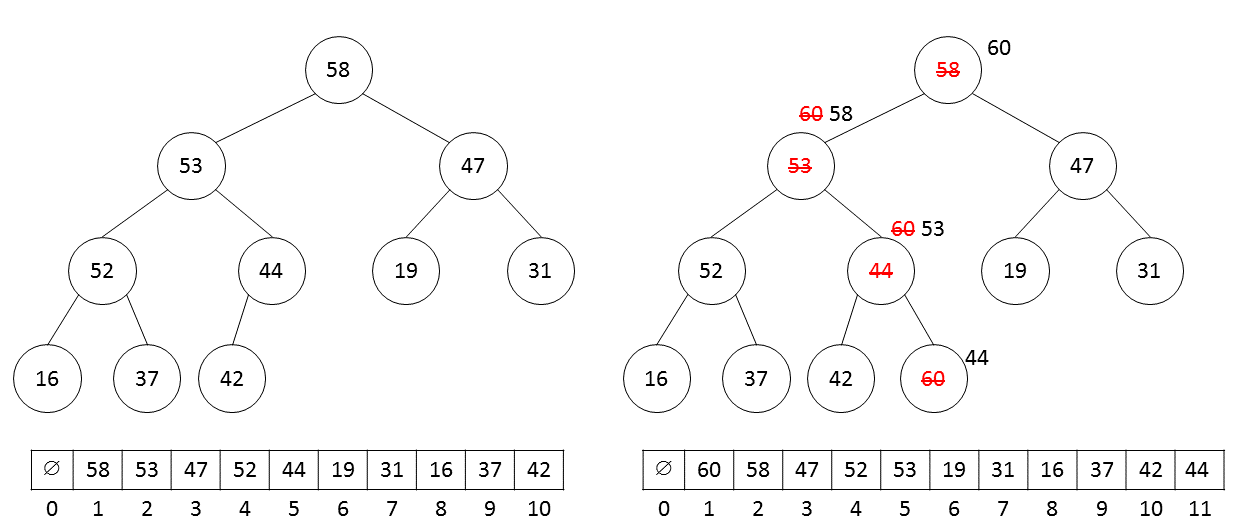
\includegraphics[width=150mm]{heap_push.png}
\caption{Εισαγωγή της τιμής 60 στο σωρό (push)}
\label{fig:heap_push}
\end{figure}


\subsubsection*{Παράδειγμα χρήσης των συναρτήσεων push και pop)}
Ο ακόλουθος κώδικας δημιουργεί σταδιακά έναν σωρό εισάγοντας δέκα τιμές με τη συνάρτηση push. Στη συνέχεια πραγματοποιούνται εξαγωγές τιμών με τη συνάρτηση pop μέχρι ο σωρός να αδειάσει.

\lstinputlisting[caption = Δημιουργία σωρού με εισαγωγές τιμών και εν συνεχεία άδειασμα του σωρού με διαδοχικές διαγραφές της μέγιστης τιμής (heap2.cpp)]{lab06/heap2.cpp}

\lstinputlisting[style=DOS]{lab06/heap2.out}


\section{Ταξινόμηση Heapsort}
Ο αλγόριθμος Heapsort προτάθηκε από τον J.W.J.Williams το 1964 \cite{nist_heapsort} και αποτελείται από 2 στάδια:
\begin{itemize}[noitemsep]
\item Δημιουργία σωρού με τα n στοιχεία ενός πίνακα που ζητείται να ταξινομηθούν. 
\item Εφαρμογή της διαγραφής της ρίζας n -1 φορές.
\end{itemize}
Το αποτέλεσμα είναι ότι τα στοιχεία αφαιρούνται από το σωρό σε φθίνουσα σειρά (για έναν σωρό μεγίστων). Καθώς κατά την αφαίρεσή του κάθε στοιχείου, αυτό τοποθετείται στο τέλος του σωρού, τελικά ο σωρός περιέχει τα αρχικά δεδομένα σε αύξουσα σειρά. 

Στη συνέχεια παρουσιάζεται η υλοποίηση του αλγορίθμου Heapsort. Επιπλέον ο κώδικας ταξινομεί πίνακες μεγέθους 10.000, 20.000, 40.000 80.000 και 100.000 που περιέχουν τυχαίες ακέραιες τιμές και πραγματοποιείται σύγκριση με τους χρόνους εκτέλεσης που επιτυγχάνει η std::sort.

\lstinputlisting[caption = Ο αλγόριθμος heapsort (heapsort.cpp)]{lab06/heapsort.cpp}

\lstinputlisting[style=DOS]{lab06/heapsort.out}

Περισσότερες πληροφορίες για την ταξινόμηση heapsort μπορούν να βρεθούν στην αναφορά \cite{programiz_heapsort}.


\section{Η δομή priority\_queue της STL}
Η STL της C++ περιέχει υλοποίηση της δομής std::priority\_queue (ουρά προτεραιότητας) η οποία είναι ένας σωρός μεγίστων. Κάθε στοιχείο που εισέρχεται  στην ουρά προτεραιότητας έχει μια προτεραιότητα που συνδέεται με αυτό και το στοιχείο με τη μεγαλύτερη προτεραιότητα βρίσκεται πάντα στην αρχή της ουράς. Οι κυριότερες λειτουργίες που υποστηρίζονται από την std::priority\_queue είναι οι ακόλουθες:
\begin{itemize}[noitemsep]
\item push: εισαγωγή ενός στοιχείου στη δομή.
\item top: επιστροφή χωρίς εξαγωγή του στοιχείου με τη μεγαλύτερη προτεραιότητα.
\item pop: απώθηση του στοιχείου με τη μεγαλύτερη προτεραιότητα.
\item size: πλήθος των στοιχείων που υπάρχουν στη δομή.
\item empty: επιστρέφει true αν η δομή είναι άδεια αλλιώς επιστρέφει false.
\end{itemize}
Ένα παράδειγμα χρήσης της std::priority\_queue ως σωρού μεγίστων αλλά και ως σωρού ελαχίστων παρουσιάζεται στη συνέχεια.

\lstinputlisting[caption = Παράδειγμα με priority\_queue της STL (stl\_priority\_queue.cpp)]{lab06/stl_priority_queue.cpp}

\lstinputlisting[style=DOS]{lab06/stl_priority_queue.out}

Περισσότερες πληροφορίες για τη δομή std::priority\_queue μπορούν να βρεθούν στις αναφορές \cite{g4g_priority_queue} και \cite{cppref_priority_queue}.


\section{Παραδείγματα}
\subsection{Παράδειγμα 1}
Χρησιμοποιώντας τον κώδικα 1, να γραφεί πρόγραμμα που να εισάγει 100.000 τυχαίες ακέραιες τιμές (στο διάστημα [-1.000.000,1.000.000]) σε έναν σωρό μεγίστων με τη συνάρτηση heap\_bottom\_up καθώς και με διαδοχικές κλήσεις της συνάρτησης push. Χρονομετρείστε τον κώδικα και στις δύο περιπτώσεις δημιουργίας του σωρού και εμφανίστε το κορυφαίο στοιχείο του σωρού. Επαναλάβετε τη διαδικασία χρησιμοποιώντας την std::priority\_queue.

\lstinputlisting[caption = Χρόνος δημιουργίας MAXHEAP: Α) με την heap\_bottom\_up Β) με σταδιακές εισαγωγές (push) τιμών στο σωρό και C) με την std::priority\_queue (lab06\_ex1.cpp)]{lab06/lab06_ex1.cpp}

\lstinputlisting[style=DOS]{lab06/lab06_ex1.out}

\subsection{Παράδειγμα 2}
Έστω ένα παιχνίδι στο οποίο οι παίκτες έχουν όνομα (name) και επίδοση (score). Να γράψετε πρόγραμμα στο οποίο να εισέρχονται στο παιχνίδι 10 παίκτες στη σειρά (player1, player2, ...), πετυχαίνοντας κάποια επίδοση ο καθένας (τυχαίος ακέραιος από το 0 μέχρι το 50.000). Να εμφανίζεται μετά την εισαγωγή του κάθε παίκτη ο παίκτης που προηγείται και η επίδοση του. Τέλος, να εμφανίζονται τα ονόματα των παικτών με τις 3 υψηλότερες επιδόσεις.

\lstinputlisting[caption = Διατήρηση επιδόσεων σε σωρό (lab06\_ex2.cpp)]{lab06/lab06_ex2.cpp}

\lstinputlisting[style=DOS]{lab06/lab06_ex2.out}


\subsection{Παράδειγμα 3}
Διάμεσος ενός δείγματος Ν παρατηρήσεων οι οποίες έχουν διαταχθεί σε αύξουσα σειρά ορίζεται ως η μεσαία παρατήρηση, όταν το Ν είναι περιττός αριθμός, ή ο μέσος όρος (ημιάθροισμα) των δύο μεσαίων παρατηρήσεων όταν το Ν είναι άρτιος αριθμός. 
Έστω ότι για διάφορες τιμές που παράγονται με κάποιον τρόπο ζητείται ο υπολογισμός της διάμεσης  τιμής καθώς παράγεται κάθε νέα τιμή και για όλες τις τιμές που έχουν προηγηθεί μαζί με την τρέχουσα τιμή όπως φαίνεται στο επόμενο παράδειγμα:\\ 
5  $\Rightarrow$  διάμεσος 5\\
5, 7 $\Rightarrow$ διάμεσος 6\\
5, 7, 13 $\Rightarrow$ διάμεσος 7\\
5, 7, 13, 12 $\Rightarrow$ 5, 7, 12, 13 $\Rightarrow$ διάμεσος 9.5\\
5, 7, 13, 12, 2 $\Rightarrow$ 2, 5, 7, 12, 13 $\Rightarrow$ διάμεσος 7

\lstinputlisting[caption = Υπολογισμός διαμέσου σε μια ροή τιμών (lab06\_ex3.cpp)]{lab06/lab06_ex3.cpp}

\lstinputlisting[style=DOS]{lab06/lab06_ex3.out}


\section{Ασκήσεις}
\begin{enumerate}
\item Να υλοποιηθεί ο σωρός μεγίστων που παρουσιάστηκε στον κώδικα 1 ως κλάση. Προσθέστε εξαιρέσεις έτσι ώστε να χειρίζονται περιπτώσεις όπως όταν ο σωρός είναι άδειος και ζητείται εξαγωγή της μεγαλύτερης τιμής ή όταν ο σωρός είναι γεμάτος και επιχειρείται εισαγωγή νέας τιμής.
\item Να γραφεί συνάρτηση που να δέχεται ως παράμετρο έναν πίνακα ακεραίων και έναν ακέραιο αριθμό κ και να επιστρέφει το κ-οστό μεγαλύτερο στοιχείο του πίνακα. 
%\item b
%\item d
\end{enumerate}

\begin{thebibliography}{9}
\bibitem{nist_heapsort}
NIST, heapsort, \href{https://xlinux.nist.gov/dads/HTML/heapSort.html}{https://xlinux.nist.gov/dads/HTML/heapSort.html}

\bibitem{programiz_heapsort}
PROGRAMIZ, Heap Sort Algorithm, \href{https://www.programiz.com/dsa/heap-sort}{https://www.programiz.com/dsa/heap-sort}

\bibitem{g4g_priority_queue}
Geeks for Geeks, Priority Queue in C++ Standard Template Library (STL), \href{http://www.geeksforgeeks.org/priority-queue-in-cpp-stl/}{http://www.geeksforgeeks.org/priority-queue-in-cpp-stl/}

\bibitem{cppref_priority_queue}
Cppreference.com, std::priority\_queue, \href{http://en.cppreference.com/w/cpp/container/priority_queue}{http://en.cppreference.com/w/cpp/container/priority\_queue}

\end{thebibliography}



\end{document}

